\documentclass{standalone}
\usepackage{amsfonts, amsmath, amssymb, bm} %Math fonts and symbols
\usepackage{dcolumn, multirow} % decimal-aligned columns, multi-row cells
\usepackage[colorlinks=true]{hyperref}
\usepackage{graphicx, subfigure, float} % graphics commands
\usepackage[margin=1in]{geometry} % sets page layout
\usepackage{setspace}% allows toggling of double/single-spacing
\usepackage{verbatim}% defines environment for un-evaluated code
\usepackage{natbib}% defines citation commands and environments.
\singlespace % set document spacing to single
\bibpunct[, ]{(}{)}{,}{a}{}{,} % sets the punctuation of the bibliography entires.
\newcolumntype{d}[1]{D{.}{.}{#1}} % defines a decimal-aligned column
\usepackage{tikz}
\usetikzlibrary{intersections}
\usepackage{enumerate}
\usepackage[utf8]{inputenc}
\usepackage[english]{babel}
\hyphenpenalty=10000

\begin{document}
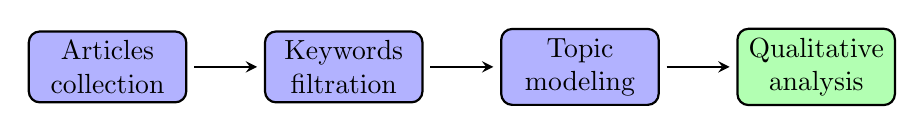
\begin{tikzpicture}[>=stealth, small/.style={
  % The shape:
  rectangle,
  % The size:
  minimum width= 2cm,
  % The border
  thick, draw=black,
      rounded corners,
      align=center}]
  \node [fill = blue!30, small] at (-3,-2.5) {Articles\\ collection};
  \node [fill = blue!30, small] at (0,-2.5) {Keywords\\ filtration};
  \node [fill = blue!30, small] at (3,-2.5) {Topic\\ modeling};
  \node [fill = green!30, small] at (6,-2.5) {Qualitative\\ analysis};

  \draw [thick, ->] (-1.9,-2.5) -- (-1.1,-2.5);
  \draw [thick, ->] (1.1,-2.5) -- (1.9,-2.5);
  \draw [thick, ->] (4.1,-2.5) -- (4.9,-2.5);
      
  \end{tikzpicture}
\end{document}
